\documentclass[11pt]{sdm}
\usepackage{xcolor}
\usepackage{float}
\usepackage[utf8]{inputenc} 
\usepackage{indentfirst}
\usepackage{listings}
\usepackage{hyphsubst}
\usepackage{amsmath}

				  
\lstdefinestyle{customc}{
  belowcaptionskip=1\baselineskip,
  breaklines=true,
  frame=L,
  xleftmargin=\parindent,
  language=C,
  showstringspaces=false,
  keywordstyle=\bfseries\color{green!40!black},
  commentstyle=\itshape\color{purple!40!black},
  identifierstyle=\color{blue},
  stringstyle=\color{orange},
}

\lstset{escapechar=@,style=customc,numbers=left}


%Number the pages
\pagestyle{plain}

\title{Software Fault Isolation using the CompCert compiler}
\author{Alexandre \textsc{DANG}}
\supervisorOne{Frédéric \textsc{Besson}}
\team{Team CELTIQUE}

\school{supelec}

\domain{Domaine: Cryptography and Security}

%write your abstract here
\abstract{}

\begin{document}
\maketitle

%*****************************************************************%

\section{Introduction}


\begin{itemize}
	\item Secure malicious code through software solution
	\item Usage in applications which use modules from unknown origin (browsers, computer clusters)
	\item current appeal for SFI speed and small TCB
	\item SFI is still incomplete, especially with ROP attack => our approach
	\item  plan
\end{itemize}


\newpage
\section{\textit{Software Fault Isolation}}
\label{sec:sfi}

	We introduce here \textit{Software Fault Isolation} (SFI) which inspired us the idea to protect return addresses through fixed stack frame size. SFI aims to protect a main program from the different modules that he will need to use. These modules will be loaded in the same memory space as the main program but in a confined area called \textit{sandbox}. The SFI mechanism is composed of two elements: a code generator and a verifier. The generator transforms the assembly code of the hazardous modules so that they will be constrained in the sandbox. The verifier operates just before loading the modules in the memory. It checks the if SFI transformations introduced by the generator are still present and valid. For the rest of the document we will reserve the word ''program'' to refer to the code protected by SFI and ''module'' to refer to the hazardous code.

\subsection{Principle}

The main principle behind SFI was first presented in the work of Wahbe and al. \textcolor{green}{ref}
. Later works \textcolor{green}{ref}, which will be introduced in the chapter \ref{ssub:Implementations}, are all based on the foundations of SFI detailed here.
The implementation described here was realised for a RISC architecture like MIPS or \textit{Alpha}.

SFI considers that a malicious code is effectively contained in the sandbox if these three security properties hold true:
\begin{itemize}
	\item \textbf{Verified code}, only instructions that have been checked by the verifier will be executed 
	\item \textbf{Memory safety}, malicious modules won't do any \textit{write} or \textit{jump} operations out of the sandbox
	\item \textbf{Flow control integrity}, every flow control transfer from hazardous modules to the main program is identified and verified
\end{itemize}
The first property protects us against self-modifying code which could bypass the SFI measures. \textit{Memory safety} prevents any illegal access to the memory of the protected program. The last property allows us to authorized only licit interactions between the program and its modules. SFI forbids any call from malicious modules that could modify the flow control of the program. If the flow control was fiddled with, it could lead to an unexpected behaviour of the program which we want to avoid.

The code generator transforms the assembly code of the hazardous modules so that respect the security properties presented before. The generator is integrated to the compiler which will create \textit{sandboxed executable}. Afterwards this executable will be checked by the verifier before being loaded in the memory. 
It verifies that the transformations introduced by the generator are present and valid. If the verification fails the module will be rejected and won't be executes. We can note that we only need to trust the verifier to prevent running any dangerous module. It's one advantage of SFI, only the verifier needs to be in the \textit{Trusted Computing base} (TCB).


\subsubsection{Code generator}
\label{ssub:Code generator}
To protect the program from its modules, the generator will restrain every write and jump instructions of the modules to addresses of their sandbox.
The generator has to face three issues to do so. Firstly, is to introduce protection mechanisms before every dangerous instructions. For example, assessing that the address of a jump instruction is an authorized one.
Secondly, we have to make sure that these protection mechanisms can't be avoided. 
Finally, the transformations introduced have to authorized only legal calls out of the sandbox by using entry points specified by the protected program. For example, Google Chrome only allows its modules to use a specific interface to interact with the browser. This way the modules can't disrupt the flow control of Google Chrome easily.
\paragraph{Confining memory accesses}
\label{par:Confining memory accesses}
The main program memory should avoid being corrupted by its modules. SFI aims to isolates these modules in a reserved of the program's memory called sandbox.
The sandbox is a contiguous memory area which size is a power of two. Indeed, these requirements eases the confinement of the modules in their sandbox by using arithmetic operations on bits which accelerates the process.
\paragraph{Protection of sandboxing mechanisms}
\label{par:Protection of sandboxing mechanisms}
\paragraph{Controlled interactions with the protected program}
\label{par:Controled interactions with the protected program}

\subsubsection{Code verifier}
\label{ssub:Code verifier}

\subsubsection{Pros and cons}
\label{ssub:Pros and cons}

\subsubsection{Implementations}
\label{ssub:Implementations}
\paragraph{NativeClient, SFI for Google Chrome}
\label{par:NativeClient, SFI for Google Chrome}


\subsection{SFI using CompCert}
\label{sub:sfi_comp}


\subsubsection{CompCert the verified compiler}
\label{ssub:CompCert the verified compiler}
\paragraph{CompCert}
\label{par:CompCert}
\paragraph{Memory model of CompCert}
\label{par:Memory model of CompCert}


\subsubsection{SFI with CompCert}
\label{ssub:SFI with CompCert}
\paragraph{Cminor}
\label{par:Cminor}
\paragraph{Specification of the SFI transformation}
\label{par:Specification of the SFI tranformation}
\paragraph{Masking in CompCert}
\label{par:Masking in CompCert}




\subsubsection{Evaluation of the approach}
\label{ssub:Evalutation of the approach}

\subsection{Limits of SFI}
\label{sub:Limits of SFI}
\subsubsection{Return addresses}
\label{ssub:Return addresses}
\subsubsection{Proposed solution}
\label{ssub:Proposed solution}


\newpage
\section{Overview of the approach}
\label{sec:Overview of the approach}
	Many attacks on software aims at diverting with the control flow of the targeted program. Among those, \textit{Returned Oriented Programming} (ROP) attacks specifically try to overwrite the return addresses.
By doing so the attacked function will return to a malicious piece of code that will get executed.
Stack overflow is an example of such ROP attacks.
We propose a solution against ROP attacks which combined with SFI would protect from most of control-flow interference attacks.
Inspired from SFI techniques we aim to prevent any overwriting of the return addresses. To do so we need to know these return addresses locations in the memory. Therefore our approach consists of modifying the stack structure in order to have a way to distinguish the return addresses locations. With this knowledge we will be able to put a mask, as in SFI, before every dangerous write instructions and prevent any ROP attack.

\subsection{ROP attack}
\label{sub:Issue}

	We want to protect our program against ROP attacks. These attacks are directed against the stack and especially the function return addresses located in the stack.
We will begin by a short introduction about the mechanisms behind the stack. Then we will explain how ROP attacks work with the example of a classical buffer overflow.

\subsubsection{The stack}
\label{ssub:The stack}
	The stack is a specific area of the memory of a program. The memory allocated to a program is divided among multiple areas like the stack (which we are going to detail), the heap (where we put dynamically allocated or global variables), the code\dots
The stack is composed of frames and each of them are linked to a function being executed. Frames are piled up on the stack following the FIFO rule (\textit{First In First Out}). Explicitly, every time a function is called, a new frame is created and placed on the top of the stack. Reciprocally when a function terminates its frame will be popped out of the stack.
Frames contain multiple kind of data related to their function like local variables, parameters of the function, return addresses... Return addresses indicates the point of execution to return to after a function terminates. When popping a frame the program is supposed to execute the code at the address matching the value contained in the return address.
ROP attacks aims to overwrite these return addresses which enables them to execute malicious code hidden in another part of the memory instead of continuing the normal flow of the program.

\subsubsection{Buffer overflow}
\label{ssub:Buffer overflow}

Stack overflows are the most popular ROP attacks. In Figure~\ref{buffer_overflow_code} we can see an example of buffer overflow written in C.
The goal of this code is to execute the function called \textit{evil\_code()} which just prints ``Argh, we got hacked!\textbackslash{n}'' line~6 of Figure~\ref{buffer_overflow_code}. We can see that in a normal execution \textit{evil\_code()} should not be executed since it is never explicitly called. 
This code was compiled with \textit{gcc -m32 -fno-stack-protector} to remove all stack protections used by gcc. The output of the code of the successful buffer overflow can be seen in Figure~\ref{output_buffer}.
\begin{figure}[!ht]
\lstinputlisting{code/buffer.c}
\centering
\caption{Example of buffer overflow in C}
\label{buffer_overflow_code}
\end{figure}

We see in the Figure~\ref{output_buffer} the consequences of the buffer overflow in red. The stack was overwritten and the return address was modified to the address of \textit{evil\_code()} which code was successfully executed.

We are going to explain how the attack works. In the function \textit{foo()} the lines~11~and~13 print the stack. \textit{\%\#010x} formats the output in hexadecimal with \texttt{0x} at the beginning for addresses.
The vulnerability resides in the function \textit{strcpy} line~12. \textit{strcpy} just copies characters one by one until it finds ``0''(which corresponds to the end of a string) in the source string. However our source string can contain many more characters than \textit{buf} is supposed to have. 
Indeed \textit{buf} is declared line~10 as an array of 1 character and our source string is the argument that we give to the program.
If the source string is bigger than the destination \textit{strcpy} will just continue to write the source string over others variables location in the stack and possibly reach the return address.
After few tries and fails we found the correct input to successfully do the buffer overflow. This input can be seen on the first line of Figure~\ref{output_buffer} which is \textit{python -c 'print 13*"a"+"\textbackslash{x7b}\textbackslash{x84}\textbackslash{x04}\textbackslash{x08}}` or \textit{aaaaaaaaaaaaa\textbackslash{x7b}\textbackslash{x84}\textbackslash{x04}\textbackslash{x08}}\\
In our example we filled the stack with ``a'' which corresponds to ``61'' in ASCII until we reached the return address.
We can see the consequence of the attack in the output Figure~\ref{output_buffer}, where the stack is full of 61 after executing \textit{strcpy}.
When we reached the return address we overwrote it with the address of \textit{evil\_code} which was \texttt{0x0804847b} given on the second line of Figure~\ref{output_buffer}.
This way, the next instruction that will be executed after \textit{foo} finishes will be the function \textit{evil\_code}.
At the end of the program we can see that we get a \textit{Segmentation fault (core dumped)}, which is normal because we messed up the stack when we overwrote is with ``a''. But since we managed to execute \textit{evil\_code} the attack is still successful.


\begin{figure}[!ht]
\textcolor{gray}{terminal\$~} ./buffer \$(python -c 'print 13*"a"+"\textbackslash{x7b}\textbackslash{x84}\textbackslash{x04}\textbackslash{x08}"') \\
\textcolor{red}{Address of evil\_code = 0x0804847b} \\
Stack before: \hfill \break
0xf7712000    \hfill \break
0xff957998    \hfill \break
0xf7593d26    \hfill \break
0xf7712d60    \hfill \break
0x0804868c    \hfill \break
0xff957978    \hfill \break
0xf7593d00    \hfill \break
0xf7713dc0    \hfill \break
0xf77828f8    \hfill \break
0xff957998    \hfill \break
0x08048510    ~~~~~~~~~~~~~~~~\textcolor{blue}{//Return address of \textit{foo}}\hfill \break
              \hfill \break
Stack after : \hfill \break
0xff958161    \hfill \break
0xff957998    \hfill \break
0xf7593d26    \hfill \break
0xf7712d60    \hfill \break
0x0804868c    \hfill \break
0xff957978   			   ~~~~~~~~~~~~~~~~\textcolor{blue}{//Buffer overflow}\hfill \break
\textcolor{red}{0x61}593d00~~~~~~~~~~~~~~~~\textcolor{blue}{//``a''   } \hfill \break
\textcolor{red}{0x61616161}~~~~~~~~~~~~~~~~\textcolor{blue}{//``aaaa''} \hfill \break
\textcolor{red}{0x61616161}~~~~~~~~~~~~~~~~\textcolor{blue}{//``aaaa''} \hfill \break
\textcolor{red}{0x61616161}~~~~~~~~~~~~~~~~\textcolor{blue}{//``aaaa''} \hfill \break
\textcolor{red}{0x0804847b}~~~~~~~~~~~~~~~~\textcolor{blue}{//"\textbackslash{x7b}\textbackslash{x84}\textbackslash{x04}\textbackslash{x08}",  \textit{evil\_code} address \\}
\\
Argh, we got hacked! ~~\textcolor{blue}{//Success! \textit{evil\_code} was executed}\\
Segmentation fault (core dumped)
\caption{Output from buffer overflow example}
\label{output_buffer}
\end{figure}


\subsection{Description of the approach}
\label{sub:Description of the approach}
	We want to protect programs against ROP attacks like the buffer overflow seen previously. We want to prevent any return address from being overwritten illegally. The only moment they should be written over is during a function call routine.
We want to be able to add runtime checks in the code like SFI, therefore we need to be able to check if an address is the location of a return address. 

The biggest difficulty is to be able to know if a location in the stack corresponds to a return address or not. Indeed the stack grows through function calls which pile up stack frames. 
These frames are constructed dynamically depending of the function, hence the locations of return addresses aren't easily known. As it is we don't have enough information to correctly protect return addresses since we don't know precisely where they are located.

Several solutions exists against this issue. We could for example add a lot of meta-data during the compilation to have extra information and then effectively protect the return addresses. Another solution is to create a second stack called \textit{shadow stack}. We would then have complete control over the \textit{shadow stack} which allows us defend against ROP attacks.
\textcolor{green}{maybe expose the cons of these approaches from our point of view}

Our solution is to modify the current stack structure to be able to know the return addresses locations easily. The main idea is to fix a constant offset $n$ between return addresses allowing us to exactly know where a return address is located relative to the others. We will explain thoroughly the approach that we want to apply in the following section.

\subsubsection{Proposed solution}
\label{ssub:Proposed solution}

\paragraph{Fixing return addresses locations and stack alignment}
\label{par:Fixing return addresses locations}

We want to be able to decide if a pointer points to a return address at runtime. With this knowledge we will be able to detect if an instruction may compromise our program.
The idea is to modify the stack layout in order to have a constant offset $n$ between neighbouring return addresses. This way we know that the neighboring return addresses are always located at a distance $n$ from a frame return address. Furthermore all the other return addresses are separated by a distance which is necessarily a multiple of $n$.
For example let's say we know the location of a return address, we call this location $c$.
Since all neighboring return addresses are separated by $n$, we know that the following return addresses locations will be $c+n$, $c+2n$\dots Reciprocally the previous return addresses will be located at $c-n$, $c-2n$\dots
Thus we have a global formula expressing the location of all return addresses: 

{\large \textbf{c~mod~n}},
with \textit{\textbf{c} the location of one of the return addresses and
\textbf{n} the size of the frames}\\

The next hurdle is to choose $n$ and $c$ cleverly. 
For $n$, the most important thing is that frames have enough space to store all the needed data. Therefore we define the value of $n$ as the biggest frame size of all the functions in a program. If the return addresses are separated by this amount we are sure that every function will have enough space in the stack for its frame. 
Afterwards we have to define $c$. The best way that we found is to modify the stack in order to have the first return addresses location to be equal to $c$. If we are able to do such a thing, we can also easily define the value of $c$ and for simplicity we chose $c=0$.

The Figure~\ref{idea_stack} pictures the transformation we want to apply to the stack. On the left we have represented an usual stack with return addresses all over the place. Since these locations are almost random it's really difficult to pinpoint their location. After transforming the stack (stack on the right) we can see that the different addresses are separated by the same constant $n$. We can also notice that we fixed the location of the first return address $c$ with the value 0.
Then we are able to know all the return addresses locations following the formula $\mathbf{0~mod~n}$.

\begin{figure}[!ht]
\centering
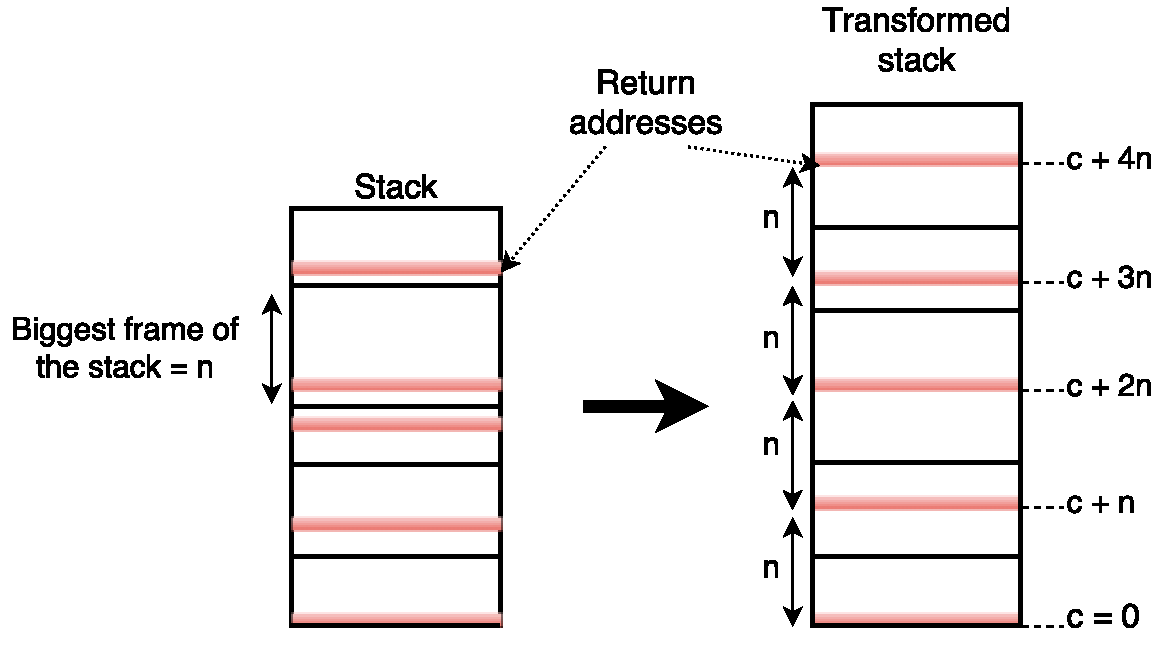
\includegraphics[scale=0.6]{images/idea_stack.pdf}
\caption{Stack modifications}
\label{idea_stack}
\end{figure}

\paragraph{Detection of dangerous instructions}
\label{par:Detection of dangerous instructions}

The second step is to detect every possibly harmful instructions to return addresses. We consider as dangerous every instruction that can freely write to the memory. Our approach is mainly related to the C language.
In C, instructions that fit such criteria are assignment to pointer dereference in the form of  \textit{(pointer)*~=~value} or \textit{(pointer+offset)*~=~value}. \\
In the previous example of buffer overflow Figure~\ref{buffer_overflow_code}, the vulnerability resides in the function \textit{strcpy} line~12. To pinpoint the dangerous instruction let's check the source code of \textit{strcpy} Figure~\ref{strcpy} from Apple.
We can see in the \textit{while} loop line~10 that \textit{strcpy} copies characters one by one from the source string \textit{s2} to the destination \textit{s} until it finds a character equals to \textit{0}.
To copy the characters, \textit{s} and \textit{s2} are pointers which initially point to the memory area of the destination and the source string. Then until it finds a character matching \textit{0} the value pointed by \textit{s2} is copied to the location pointed by \textit{s} and the pointers are incremented. The harm happens when the source \textit{s2} is much longer than the destination. In this case we continue to copy to the location pointed by \textit{s} even if the memory written to does not belong to the destination string anymore.\\
In this example we see clearly that it's the pointer dereferencing that allows one to write directly in the memory. For that reason we target such type of instructions in our approach.

\begin{figure}[!ht]
\begin{lstlisting}
char * strcpy(char *s1, const char *s2) {
	char *s = s1;
	while ((*s++ = *s2++) != 0)
		;
	return s1;
}
\end{lstlisting}
\centering
\caption{\textit{strcpy} source code from Apple}
\label{strcpy}
\end{figure}

\paragraph{Securing dangerous statements}
\label{par:Protection around dangerous statements}

Finally when we have detected all the dangerous statements we transform the module code. Before each of this dangerous statement we add a protection mechanism similar to masking in SFI. The algorithm of the check is represented in Figure \ref{runtime_check}: \\
	\begin{enumerate}
		\item We check if the address is in the stack. Return addresses only exist in the stack, we don't need to concern ourselves with the other accessible memory area: the heap.
		\item If the address is in the stack we check if the target address matches our formula \textbf{0~mod~n}. If it does then it's a return address location.
		\item If a target address abides by the two previous condition, it's an illegal instruction and we make the program crash. If it does not then the program just continue to run like normal.
	\end{enumerate}
We want our implementation to respect the property of transparency, if a program is safe then our transformation does not modify its behaviour.

\begin{figure}[!ht]
\centering
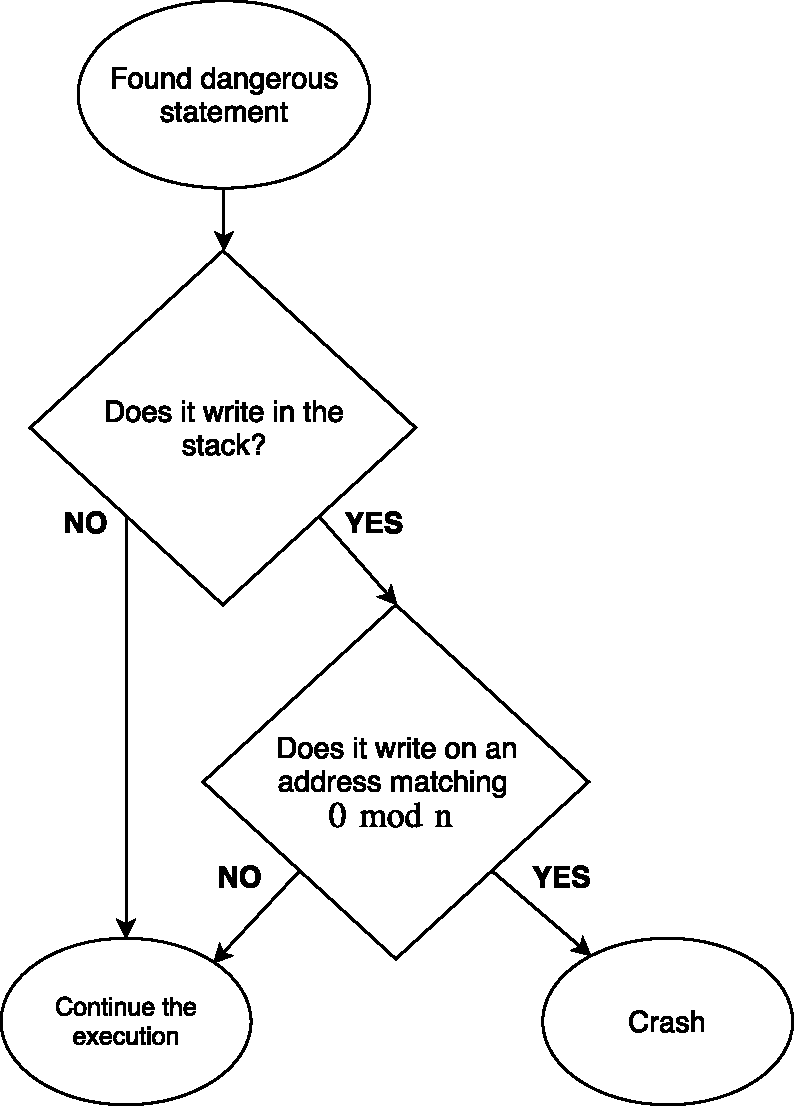
\includegraphics[scale=0.6]{images/runtime_check.pdf}
\caption{Runtime check algorithm}
\label{runtime_check}
\end{figure}

\hfill \break 
	To sum it up, our approach aims to have an easy way to know return addresses location and then add a check at runtime before every dangerous instruction to prevent illegal writing on return addresses location.
To do this we divided the approach into four phases:
\begin{enumerate}
	\item Fix stack frames size
	\item Align the stack
	\item Detect dangerous statements
	\item Secure the dangerous statements
\end{enumerate}


\subsection{Security properties}
\label{sub:Security properties}
	The approach we propose is composed of four phases, to get the confidence that our idea is effective in protecting return addresses we are going to formalize the properties we expect from each phase. 
Furthermore like we pointed earlier, we are going to work with the certified compiler CompCert.
The ideal way to be sure of our idea would be to prove it with Coq the proof assistant the language used to build CompCert.
By working with these tools we hope that one day we will be able to prove some security guarantees brought by our approach.

\begin{enumerate}
	\item \textbf{Fixed stack frames size}
		\begin{itemize}
			\item Return addresses locations are all separated by a constant offset bigger or equal to any frame of the stack
		\end{itemize}
	\item \textbf{Stack alignment}
		\begin{itemize}
			\item The first return address location of the program has its least significant bits equal to 0
		\end{itemize}
	\item \textbf{Detection of memory write statements}
		\begin{itemize}
			\item Every statement of the analysed code that might modify the stack memory state is detected
		\end{itemize}
	\item \textbf{Securing memory write statements}
		\begin{itemize}
			\item The protection will trigger an error behaviour if we try to write on a protected address
		\end{itemize}
\end{enumerate}

1. and 2. combined give us the guarantee that the least significant bits of all the return addresses location will be equal to $\mathbf{0~mod~n}$ with $n$ the fixed offset between return addresses.
Basically we make it so the protection mechanism prevents any write on addresses located in the \textbf{stack memory area} with their least significant bits equal to $\mathbf{0~mod~n}$.

\hfill \break 
Another property we didn't mention yet is that all our transformations need to be transparent. In other words, if we apply our methods on a program which is already safe then its behaviour is not affected. We will explain how we ensure this property more thoroughly in the Chapter~\ref{sec:implementation}.

\hfill \break 
For these properties to always hold true we need to place some conditions which we are going to list in the following section. Our approach guarantees that if all the properties mentioned are fulfilled the program will be protected against any ROP attack.

\subsection{Analysis of the approach}
\label{sub:Analysis of the approach}

\subsubsection{Conditions}
\label{ssub:Conditions}

The solution we've just presented can bring very strong security properties against ROP attacks. However for this approach to work we need certain hypothesis to be true. Indeed some of the properties enumerated before become false after certain operations.

\begin{itemize}
	\item \textbf{Stack modifications}, every operation that disrupts the stack structure may nullify our property that says ''every return addresses are separated by a fixed offset''. For example x86 architecture use the ESP register to keep track of the stack growth. If we fiddle with it we may introduce a shift in the return addresses location. Then our runtime check on $\mathbf{0~mod~n}$ addresses would not be relevant anymore.
		For example, the Figure~\ref{inline_assembly} shows a piece of inline assembly which disrupts the stack line~2. Inline assembly allows one to put some assembly code in the middle of C code. Here the assembly decrements the stack pointer stored in ESP. By doing so the stack will be shifted by an amount of 50 bytes and our formula to the locations of return addresses won't be correct anymore.

	\item \textbf{Unsecure libraries}, for our approach to work we need to have all dangerous write statements to contain our runtime checks. Hence all executed code must have been compiled with our transformation. For example, the \textit{glibc} library of C contains multiple insecure functions like \textit{printf, strcpy\dots} Furthermore those flawed functions are common vulnerabilities for \textit{buffer overflows} attacks which are a type of ROP attack. To avoid this issue we would need to rewrite the glibc or compile it with our tools.

	\item \textbf{Modules need the same offset}, if a program uses multiple modules or library they need to be compiled with the same offset $n$. Indeed if the offset of the different modules are different we cannot use the previously defined formula $\mathbf{0~mod~n}$ cannot be used anymore. Thus it's not possible to easily know if a location corresponds to a return address.
\end{itemize}

\begin{figure}[!ht]
%asm(''sub $50, %esp'');
\textcolor{green}{TODO substitute with the right syntax when finished}
\begin{lstlisting}
int foo(int a) {
	asm(``\$sub 50, \%esp'');
	//This line does the operation ESP = ESP - 50
	//This disrupts the stack layout we establish in our transformation
	printf("Hello world!");
}
\end{lstlisting}
\centering
\caption{C inline assembly}
\label{inline_assembly}
\end{figure}

\subsubsection{Discussion}
\label{ssub:Discussion}
	We have presented the principle of our approach in this chapter. Then we mentioned some necessary conditions for our solution to work properly. In this section we are going to discuss about the pros, cons or remarks about the proposed solution.

	The benefits of our transformation is clear, any code compiled with a compiler enforcing our methods is unable to interfere with the control flow of our program through return addresses.
	Furthermore if we combine our solution with the SFI presented earlier we can have some strong security properties on the execution of dangerous modules with our main program.
Alas there are also some disadvantages to our approach that we are going to present here:
	\begin{itemize}
		\item \textbf{Architecture dependant}, our solution depends a lot of the stack layout of the program. Indeed fixing the size of the frames requires us to modify the original stack layout. Therefore since the stack layout vary depending of the architecture and compiler you are using, the modifications that have to be done are also different. We can then easily comprehend that we would need a different implementations for every existing stack layout. Moreover since these layouts can be really different it might be very gruesome to implement our solution on certain of them.
In the implementation we present after we focus solely on x86-32 architecture with the compiler CompCert.
		\item \textbf{Memory consumption}, since we are fixing the size of the frames instead of having dynamic sizes the memory usage of the stack is bigger. We have the issue of choosing an adequate size for the frames in our solution. The easiest one is to take the maximum frame size of the program as the constant size for all the frames. The downside is that we might have a memory usage explosion from our stack.
We didn't encounter any issue about memory during the tests we did but the impacts may be visible on especially big programs. It might be interesting to study the cost of our approach on the growth of the stack.
	\end{itemize}

Despite the cons presented we believe the benefits we gain from this method is worth it.
We are going to present in the following section the implementation we made based on the ideas we introduced here. This implementation was made with the compiler CompCert for the x86-32 architecture. We are targeting programs written in C, which explains that all the examples we used were related to the C language.


\newpage
\section{Implementation}
\label{sec:implementation}

For the implementation of our idea we chose to work with the compiler CompCert. CompCert already had an implementation of SFI presented earlier. Thus if we could combine our approach with the SFI, any program compiled with CompCert would have strong security guarantees. Furthermore CompCert is written with Coq the proof assistant, we eventually hope that we will be able to prove these security properties. In this section we are going explain in details how we implemented the approach and the different choices we did during the process. Afterwards we will discuss these choices and evaluate the results and performance obtained.

\subsection{Implementation}
\label{sub:Implementation}
	Our approach is separated in four phases: ``Fixed stack frames size'', ``Stack alignment'', ``Detection of memory write statements'' and ``Evaluation of the implementation''. We are going to detail the implementation of these phases in the following sections. These transformations are deeply linked to the stack layout, hence to have a better understanding we are going to start by introducing the CompCert stack structure.

\subsubsection{CompCert stack}
\label{ssub:CompCert stack}
	The layout of the stack is dependent of the architecture and the compiler/interpreter used. For the sake of comprehension of the future sections we describe here the stack layout of x86-32 in CompCert.
The stack layout of CompCert x86-32 is pictured in Figure~\ref{stack_layout}.
First of all we can notice that the stack grows downwards, it means that the stack grows from the highest addresses to the low ones.
As we can see the usual data are stored in this stack like local variables, parameters, register states and the return address.

\begin{figure}[!ht]
\centering
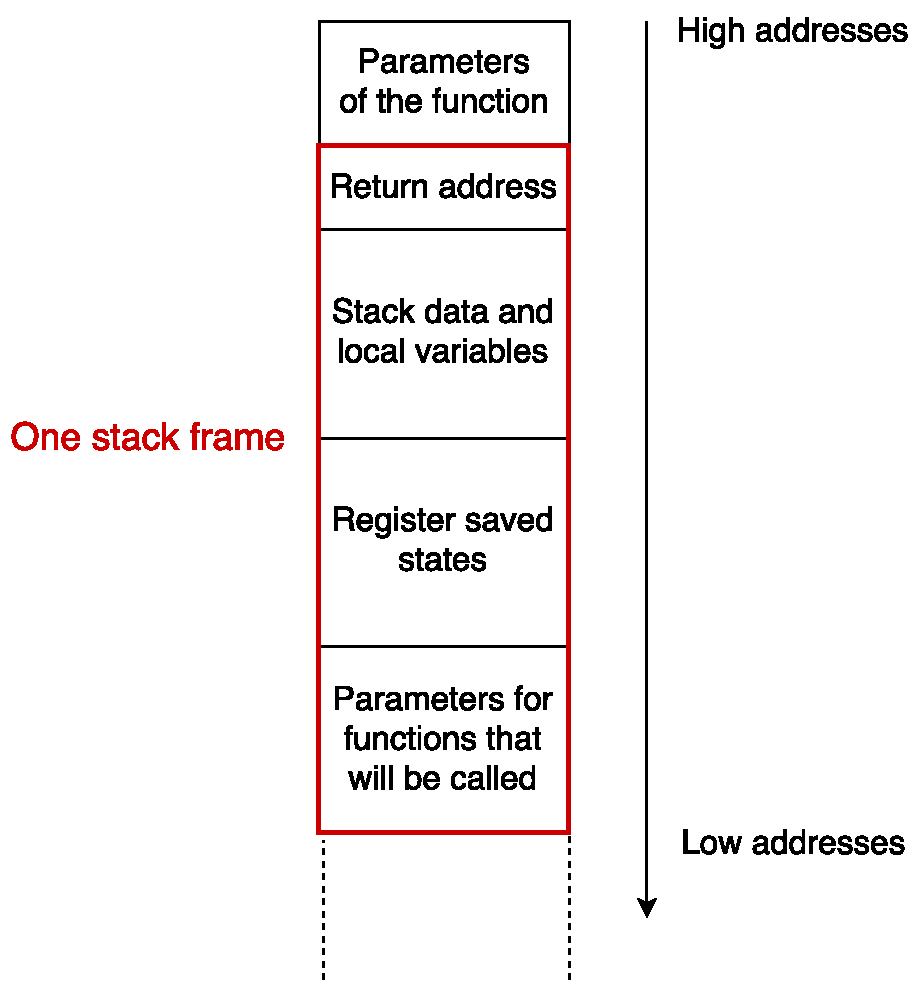
\includegraphics[scale=0.55]{images/stack_layout.pdf}
\caption{CompCert x86-32 stack layout}
\label{stack_layout}
\end{figure}

Each frame is built when a function is called, the different steps related to the creation of a frame is called \textit{function call routine}.
CompCert function call routine is described in the Figure~\ref{call_routine}. Each phase of the function call routine of the Figure~\ref{call_routine} is explained just here:
\begin{enumerate}
	\item Write the return address
	\item Allocate enough memory for the rest of the stack
	\item Save registers states in the stack
	\item Execute the function body (use the memory for local and stack data)
	\item When calling another function, place its parameters at the end of the stack and repeat the process
\end{enumerate}

\begin{figure}[!ht]
\centering
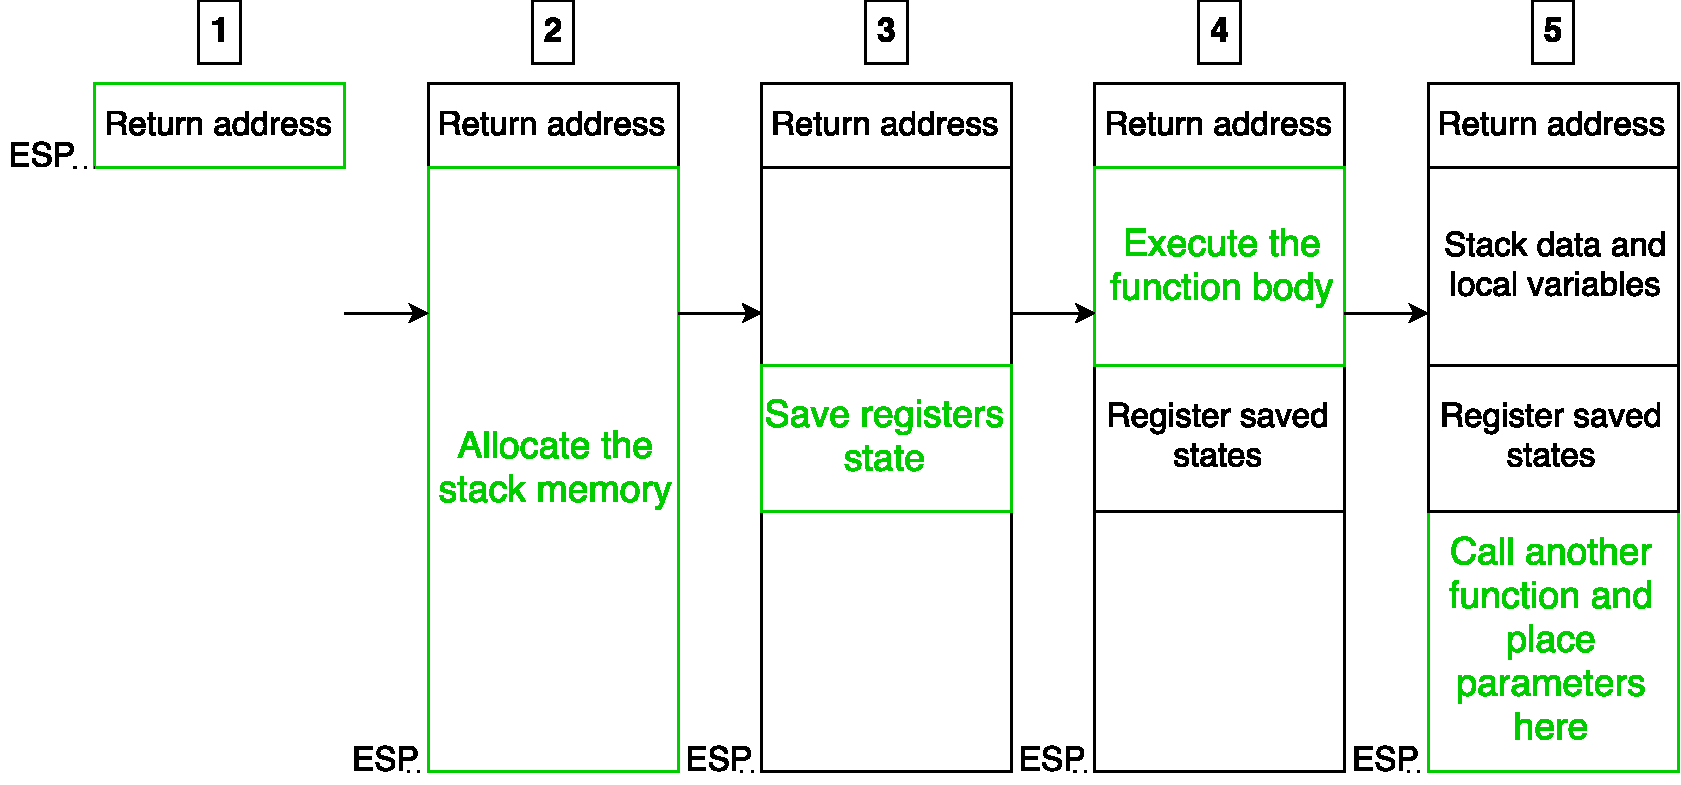
\includegraphics[scale=0.55]{images/call_routine.pdf}
\caption{CompCert function call routine}
\label{call_routine}
\end{figure}

When returning from a function, the return routine is pretty much the opposite:
\begin{enumerate}
	\item Restore registers state
	\item Deallocate the stack until the return addresses
	\item Pop the return address memory and jump to the value stored in it
\end{enumerate}


\subsubsection{Fixed stack frames size}
\label{sub:Fixed stack frames size}
During this phase we want to ensure these two properties:
\begin{itemize}
	\item Return addresses locations are all separated by a constant offset bigger or equal to any frames of the stack
\end{itemize}

\paragraph{Fix the frames size}
\label{par:Fix the frames size}

Fortunately in the function call routine of CompCert the return addresses are always at the top of their frames.
This particularity makes the task easier, indeed, since the location of the return address is fixed in the stack we can simply fix the size of the frames to have a constant offset between the return addresses. 
This special trait is not always true, for example in x86 architecture with the compiler \textit{gcc} the location of the return addresses changes relatively to the frame depending of the parameters of the function.

To fix the size of stack we had to find the description of the stack in CompCert. Then we just had to put a constant in the attribute \textit{size} of the stack and readjust the alignment of the different parts of the frames. We told CompCert to keep the return address of the stack as the first location in the frame and that all the extra space introduced by the fixed size will be taken for  \textit{stack data and locals}. The remaining parts keep the same alignment as before.

\paragraph{Choice of frames size}
\label{par:Choice of frames size}

We chose to limit the choice of the frames size to powers of two. Indeed, since addresses are written in binary having a power of two as constant offset will ease the runtime checks implementation. Indeed by using powers of two, all the return addresses will have the same least significant bits. For example if the first return address location is \texttt{0xffffff911} (in hexadecimal) and our constant frame size is $2^8 = \texttt{100}$ (in hexadecimal). Then all the following return addresses locations will be \texttt{0xfffff811} (the stack grow downwards), \texttt{0xfffff711}, \texttt{0xfffff611}\dots And their least significant bits are actually always equal to \texttt{11}. This particularity will help during the phase of runtime checks that we will explain in section~\ref{ssub:implem_check_address}.

To prevent having compiled programs with too small stack frame, we added in CompCert a check. This test verifies that the chosen size is bigger than any dynamically calculated one. If it's not, the compilation fails. This way the chosen size corresponds to \textbf{the smallest power of two which is bigger or equal to any dynamically calculated frames size of the program}.

We can see in Figure~\ref{stack_transform} the effect of our implementation. 
The left stack is the usual layout of CompCert stacks with the return addresses located at the top of the frames. We call $F_{size}$ the size of the biggest frame of the whole program.

For our transformed stack we have to chose a fixed size for the frames and it needs to be a power of two, bigger or equal to $F_{size}$. In Figure~\ref{stack_transform} we chose $2^8$ to continue the examples we gave before.
We can see that the stack on the right has fixed size frames equal to $2^8$ and the return addresses are all separated by the same offset dues to CompCert stack layout.
The implementation effectively fulfills the property of having constant offset between return addresses.
Furthermore we can see that the location of the return addresses are \texttt{0xfffff911}, \texttt{0xfffff811}, \texttt{0xfffff711}\dots
Hence all the return addresses have the particularity of always having the same least significant bits (\texttt{11}). This particularity will be used later for the implementation of the protection mechanism.

\begin{figure}[!ht]
\centering
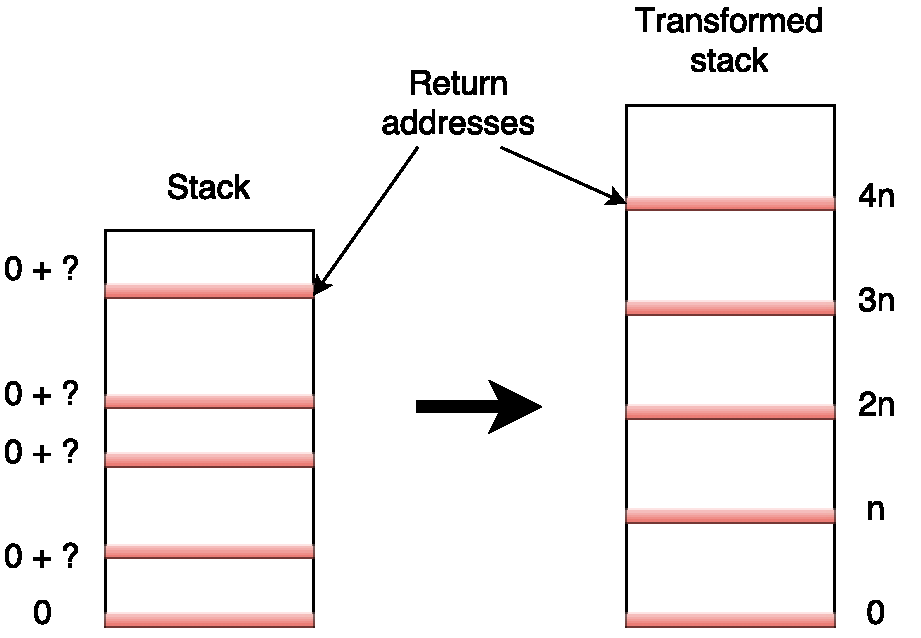
\includegraphics[scale=0.6]{images/stack_transform.pdf}
\caption{Fixing the size of CompCert stack frames}
\label{stack_transform}
\end{figure}

\subsubsection{Stack alignment}
\label{ssub:Stack alignment}

The implementation in this section has to do a transformation that makes the following property true:
\begin{itemize}
	\item The first return address location of the program has its least significant bits equal to 0
\end{itemize}

We had multiple choices for the implementation of this property. One of them was to modify the main function of the protected program in order to align the return addresses locations correctly. Another idea was to modify the prelude of a program, the prelude is a piece of code created by the compilers which is executed before the program. It is necessary for any program to have this prelude to work correctly.

Eventually we chose to introduce before the \textit{main} function of the program an artificial \textit{main}. Its role is to align the stack in order to make all the incoming return addresses locations to match our formula $0~mod~n$. 
This approach has one definite advantage over the others solutions listed before. Creating a whole new function prevents us to modify recklessly core parts of the program like the original \textit{main} or the prelude. \hfill \break

Since we have to modify the stack structure we did our transformation at the assembly level(ASM). Indeed the stack pointer ESP which is responsible for the stack growth is only available in ASM. ASM is the lowest level before binary code, though it is difficult to modify ASM correctly since you have to manipulate low level objects. 
By creating a separate artificial \textit{main} function we avoid taking the risk of bugging the prelude or the program's \textit{main} function.

Figure~\ref{stack_align} represents the stack alignment transformation. The left stack is CompCert stack with fixed frames size equal to $n=2^8$ like we had in the previous section. From this stack we show the consequences of our operation. We insert before the \textit{main} function of the program an artificial \textit{main}. Thus the frame of this artificial \textit{main} is the first frame of the whole stack. The artificial \textit{main} objective is to align the stack in order to have the next return address equal to \textbf{0~mod~n}. \\
We can see on the left stack the effect of the transformation. The return address of \textit{main} was previously at the address \texttt{0xfffff911} and is now at \texttt{0xfffff700}. Since the frames size remained constant we now have all the following return addresses locations matching \textbf{0~mod~n}. This was the objective of the whole stack transformation which is now completed.
The downside of this implementation can be seen clearly on the Figure~\ref{stack_align}. Indeed all the return addresses locations are equal to \textbf{0~mod~n} except the return address of the artificial \textit{main} we introduced.
Since our approach aims to protect the locations matching \textbf{0~mod~n}, this return address is vulnerable.
Nevertheless, to reach this location an attacker would need to either know the exact location either overwrite the whole stack.
\begin{itemize}
	\item To pinpoint the location of vulnerable return address is really difficult, it would requires a lot of tries and fails or luck. Furthermore, nowadays most of the systems have a security feature called ASLR which inserts randomness in the memory addresses like the stack location. It means that every time a program is executed the location of this return address will be different which complicates the attack. Another possibility is to add in our runtime checks an extra condition to protect this specific return address.
	\item The other way to reach this unprotected return address is prevented by our implementation. The attacker would need to overwrite other frames return address to reach the vulnerable one. In this case our approach will make the program crash before it can arrive at the artificial \textit{main} frame.
\end{itemize}

\begin{figure}[!ht]
\centering
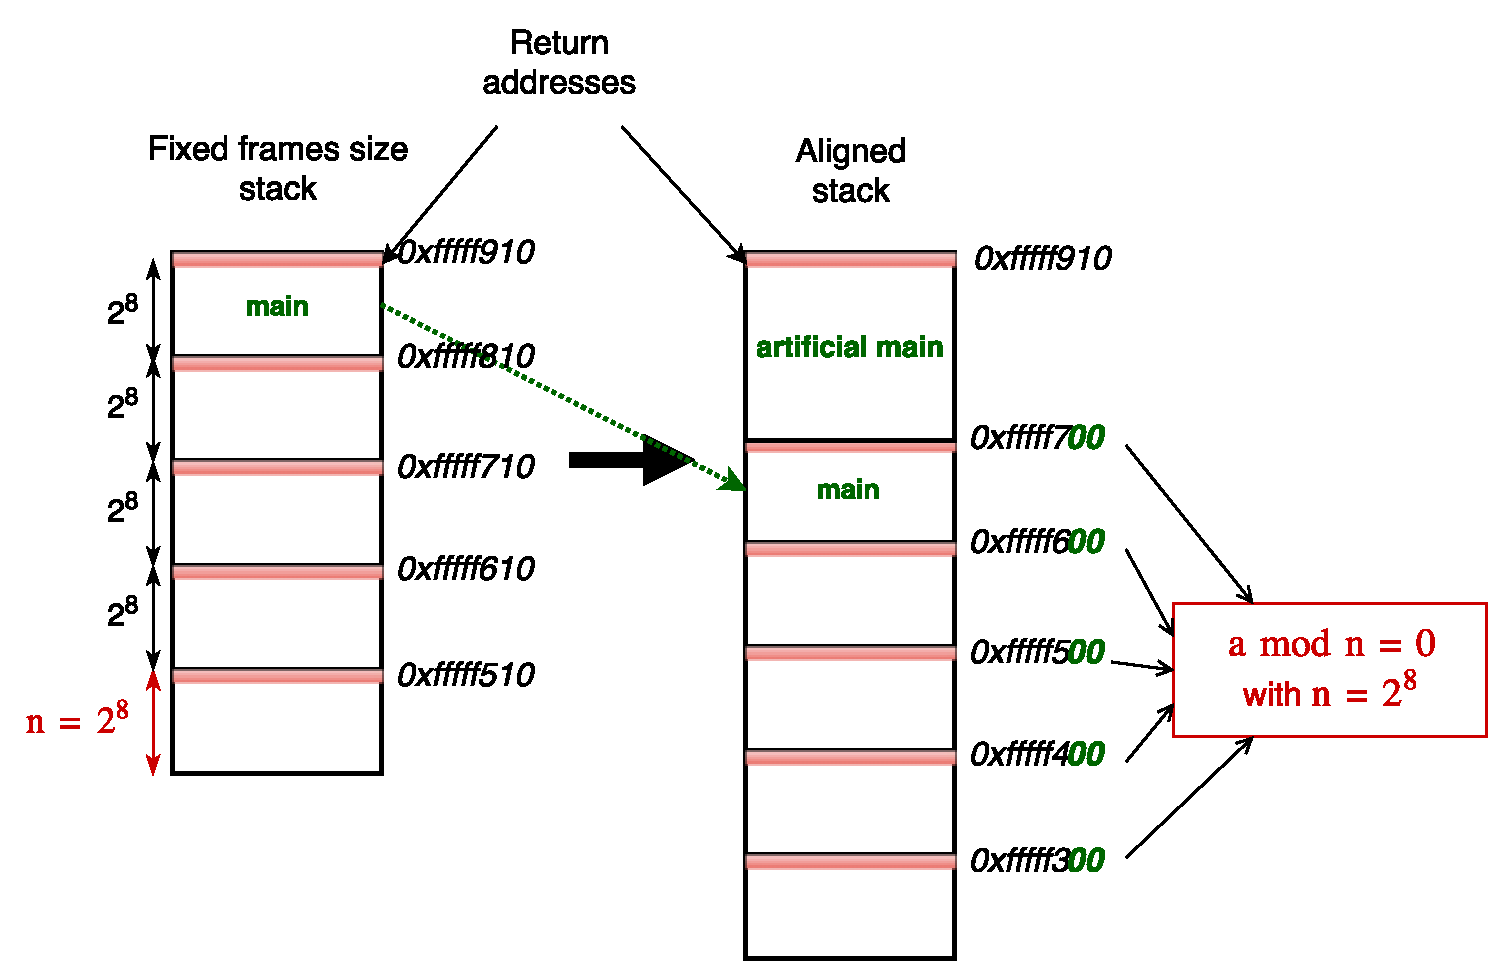
\includegraphics[scale=0.6]{images/stack_align.pdf}
\caption{Aligning CompCert stack frames}
\label{stack_align}
\end{figure}

\paragraph{Alignment algorithm}
\label{par:Alignment algorithm}
We present in Figure~\ref{align_algo}, the algorithm used to calculate the right size in order to have the next return addresses aligned. The algorithm is written in pseudo assembly code.

The easiest way to understand it is to go through it with an example. On the previous examples Figure~\ref{stack_transform} and Figure~\ref{stack_align} our stack started at the value \texttt{0xfffff911}. Hence for the continuity we will keep this value. In Figure~\ref{stack_align} we want to have our next frame starting at the address \texttt{0xfffff700}. We go through the different lines of Figure~\ref{align_algo} to explain the algorithm:
\begin{enumerate}
	\item we copy the current \textit{next\_frame} location into a register called \textit{reg}, for the example we take randomly \textit{next\_frame} =  \texttt{0xfffff840}.\\
		The operation is then \textit{reg} = \textit{next\_frame} = \texttt{0xfffff840}
	\item \textit{reg} = \textit{reg} \& $(n-1)$ = \texttt{0xfffff840} \& \texttt{0x000000ff} = \texttt{0x00000040}\\
		In our examples we have $n-1 = 2^8-1$ = \texttt{0x000000ff}
	\item \textit{reg} = \textit{reg} $+(n-4)$ = \texttt{0x0000040} $+$ \texttt{0x000000fc} = \texttt{0x00000140}
	\item \textit{next\_frame} $=$ \textit{next\_frame} $-$ \textit{reg} = \texttt{0xfffff840} $-$ \texttt{0x00000140} $=$ \texttt{0xfffff700}
	\item We start the function call routine, here we save registers state in the stack
	\item We store the parameters of the original \textit{main} in the stack
	\item We call the original \textit{main} function, its frame will start at the location stored in \textit{next\_frame}~$=$~\texttt{0xfffff700}
\end{enumerate}

A small remark on the example is that our algorithm only works if the last bit of the first value of \textit{next\_frame} = \texttt{0xfffff840} is \texttt{0}. However this particularity is already present in all compilers since it improves the speed of execution and then our algorithm works with all standard addresses.
\begin{figure}[!ht]
\centering
\begin{lstlisting}
move	reg		next_frame  
and	reg		n-1	    
add	reg		n-4    
sub 	next_frame	reg
store 	regs_state
store	parameters
call	main
	
\end{lstlisting}
\caption{Alignment algorithm}
\label{align_algo}
\end{figure}

\subsubsection{Detection of memory write statements}
\label{ssub:Detection of memory write statements}
We have to make sure that we cover all possibly harmful statements with our runtime protection. Since we are working with the compiler CompCert we are going to take advantage of it. CompCert has multiple compilation steps which have all been proven from C to assembly language. To prove these steps for each step language a semantic was defined in relation to the memory model briefly described in section~\ref{sub:sfi_comp}.
To detect all dangerous statements we looked at the semantic of Clight and found all statements that in the memory model could access freely the memory.\\
We chose Clight to implement the detection of dangerous statements and also for the runtime protection of those. This choice is explained by the fact that Clight is a high-level language. 
Indeed doing our transformations at a high-level is much easier since all the complicated compilation operations are done later in the process. For example by using Clight we don't need to bother with low-level objects like registers. Furthermore Clight is a compilation step placed before any optimizations. This mean that our transformations can be optimized automatically by CompCert which can improve our performances.

\subsubsection{Securing memory write statements}
\label{ssub:implem_check_address}

\subsection{Evaluation of the implementation}
\label{sub:Evaluation of the implementation}





\end{document}
%%% Local Variables:
%%% mode: latex
%%% TeX-master:
%%% End:

